\section{Face representation and identification}
Approaching the face recognition challenge, we gave up manually crafted features as LBP or HOG in favour of more sophisticated ones learned by deep learning methods in a data driven way. Therefore, we employed a solution respecting the FaceNet system which, based on  deep convolutional neural network architecture, learns the mappings of faces on an 128-dimensional euclidian space where the simple L2 norm represents the similarity between faces. In order for such a system to be reliable it should prove that is, among others, pose and ilumination invariant, as well as scale, that is not prone to errors due to the quality of the image and also should be able to match faces in photos took years apart. For a lot of these challenges, the FaceNet system managed to find a way to overcome them as Schroff et all. presented in \cite{SchroffKP15}.
\begin{figure}[h]
	\begin{center}
		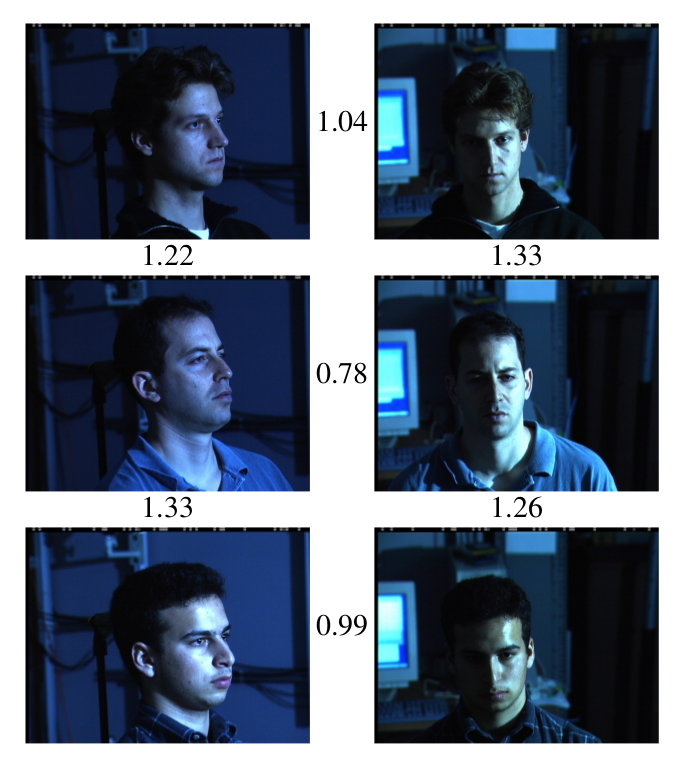
\includegraphics[width=7cm]{facenet-results}
	\end{center}
	\caption[FaceNet pose and ilumination invariance from \cite{SchroffKP15}]{Results presented in \cite{SchroffKP15} regarding the pose and ilumination invariance of the FaceNet system. As can be observed, there is a significant difference in distance between faces on the same line corresponding to the same identity and faces on different lines.}
\end{figure}
\subsection{Triplet loss}
As already stated, the FaceNet system is based on a convolutional neural network architecture. Treating the model details as a black box, the task required a form of evaluation that would reflect the desired result in the matter of face verification, recognition and clustering. As described in \cite{SchroffKP15} the target was to find an embedding $f(x)$ defined on the space of face images and into a feature space $\rm I\!R^{d}$ where the square distance between all images of the same face to be small regardless of imaging conditions and large between images of faces corresponding to different identities. Another constraint on $f(x)$ was to live on the $d$-dimensional hypersphere, meaning $||f(x)||_{2}=1$. As opposed to other losses, the triplet loss does not try to enforce the embedding on a single point but conducts the mapping of the same identity faces on a manifold while still allows a discriminative distance between faces of different identity. 

In other words, the purpose of the triplet loss is to ensure that an anchor image $x_{i}^{a}$ of a face is closer to all other images of the same face $x_{i}^{p}$ than any other image of different identity face $x_{i}^{n}$. This can be written as
\begin{align}
	||x_{i}^{a}  - x_{i}^{p} ||_{2} + \alpha < ||x_{i}^{a}  - x_{i}^{n} ||_{2} \forall (x_{i}^{a}, x_{i}^{p}, x_{i}^{n}) \in \Psi
\end{align} where $\Psi$ is the set of all triplets from the training data.

\subsection{CNN architecture}

\subsection{Face identification}